\documentclass{article}
\usepackage[utf8]{inputenc} % allow utf-8 input
\usepackage[T1]{fontenc}    % use 8-bit T1 fonts
\usepackage[hidelinks]{hyperref}       % hyperlinks
\usepackage{url}            % simple URL typesetting
\usepackage{booktabs}       % professional-quality tables
\usepackage{amsfonts}       % blackboard math symbols
\usepackage{nicefrac}       % compact symbols for 1/2, etc.
\usepackage{microtype}      % microtypography
\usepackage{graphicx}
\usepackage{subcaption}
\usepackage[margin=0.8in]{geometry}
\newcommand\tab[1][0.5cm]{\hspace*{#1}}

\title{3D Fully Convolutional U-Net Approaches to Brain Tumor Image Segmentation}

\author{
  Cameron Backes and Jonathan Deaton\\
  Stanford University\\
  \{cbackes,  jdeaton\} @stanford.edu\\
  }

\begin{document}

\maketitle
\begin{abstract}
\noindent This project explores the application of 3D fully-convolutional deep networks for brain tumor segmentation tasks in magnetic resonance images (MRIs). We created, trained, and tested three variant models of the U-net architecture using the dice coefficient as our primary performance metric to assess the overlap between predicted and ground-truth segmentations. We trained and tested our models using datasets from the 2018 Brain Tumor Segmentation (BraTS) \cite{BraTS,BraTS2} challenge, and were able to achieve whole tumor segmentation performance, as indexed by dice score, that is on par with the state-of-the-art from recent years. 
\end{abstract}

\section{Introduction}	
\tab Noninvasive methods of brain imaging, most commonly magnetic resonance imaging (MRI), are routinely used to identify and locate tumors in the brain. Currently, brain tumor image segmentation is a time consuming practice, which must be performed manually by medical professionals. As such, with the recent emergence of effective computer vision methods, notably convolutional neural networks (CNNs), there is significant societal value in using these tools to automate and improve the accuracy of segmentation for a variety of medical applications, particularly for deployment in regions where medical personnel are sparse. We have created, trained, and tested three models using a 3D Fully Convolutional U-net architecture that take as input a 3D MR image of a tumor-containing brain, and outputs a predicted tumor segmentation, as a part of the 2018 Brain Tumor Segmentation (BraTS) challenge \cite{BraTSData}. Our best model achieved an average Dice coefficient of .87 on our test set, making our model’s performance on par with state-of-the-art performance from recent years’ BraTS challenges.

\section{Related work}
\tab Until recently, discriminatory models such as random forest and support vector machines (SVMs), as well as graphical models such as hidden Markov models (HMMs) were the most commonly used and most effective methods for semantic image segmentation. However, over the past few years, convolutional neural networks have emerged as the state of the art technique for brain tumor image segmentation \cite{DBLP:journals/corr/HavaeiDWBCBPJL15, Shelhamer, DBLP:journals/corr/NovikovMLHWB17}, as index by dice coefficient, the most commonly accepted metric for assessing the degree overlap between the predicted and ground-truth segmentations. Furthermore, the use of fully convolutional neural networks, which lack a dense, fully connected output layer have been shown to achieve results comparable to models with dense layers with significantly less computational cost \cite{Shelhamer}. Amongst emerging CNN architectures for semantic image segmentation, the U-Net architecture, which contains symmetric down-sampling layers to capture image context and up-sampling layers to capture precise feature localization, has been demonstrated to achieve stellar segmentation performance even when given a small number of image inputs \cite{DBLP:journals/corr/RonnebergerFB15}. As such, this technique is particularly well suited to biomedical image segmentation, where even the largest available datasets are typically on the order of hundreds to thousands of images, which is far too small for most CNNs. Furthermore, the U-Net architecture is fully convolutional and as such is able to perform segmentation much more efficiently than alternative architectures that utilize dense layers \cite{DBLP:journals/corr/RonnebergerFB15}. Most of the existing approaches that have used CNNs, and U-Nets in particular, for image segmentation of 3D biomedical images have used 2D images slices rather than incorporation of the entire 3D image input; however, when 3D models have been applied they have achieved superior results \cite{DBLP:journals/corr/KamnitsasLNSKMR16}, despite increased computational demands. 

\section{Dataset and Features}
\tab The 2018 Brain Tumor Segmentation (BraTS) dataset was collected by medical professionals from numerous institutions, notably UPenn’s Center for Biomedical Image Computing and Analysis (CBICA). It consists of 3D MRI brain scans from 285 individuals with brain tumors, along with age and survival information for each individual, and ground-truth tumor segmentation labels for tumor voxels manually-revised by expert board-certified neuroradiologists. Each MRI scan corresponds to a single individual and consists of 4 different image modalities: T1, T1-enhanced, T2, and T2-FLAIR, and for each scan type there is a $(240 \times 240 \times 155)$ voxel 3D gray-scale image input, where each voxel represents a feature in our model. The accompanying ground-truth segmentation for each MRI scan is a single $(240 \times 240 \times 155)$ voxel image where non-tumor voxels are labeled $0$ and tumor voxels are labeled $1, 2,$ and $4$ depending on the severity of the tumor in that region.

We randomly split the data into a training set with 205 images, a validation set with 40 images, and a test set with 40 images, and converted the images into the TFRecord format for efficient loading into TensorFlow. We then performed several steps of data-preprocessing so that the input would be suitable for the model. Because we were doing whole-tumor segmentation, the first pre-processing step was to convert all segmentation labels to either a zero or a one designating non-tumor and tumor, respectively. Other steps of preprocessing involved combining each of the four image modalities into a single four-channel 3D volume, and cropping each MRI and segmentation mask.

Furthermore, we augmented our training dataset by flipping each image along all 3 axes, thereby expanding the effective dataset size by a factor of four. We also attempted to add gaussian noise and gaussian blurring to the images for additional augmentation but struggled to apply these transformation with the proper amplitude and they did not end up being used to train any of the models. Because we utilized TensorFlow's Dataset API, pre-processing and augmentation were performed in parallel with training, and therefore more efficiently utilized the machine's resources at training time. This also bought the advantage of not having to store the duplicated data on disk and instead merely needed to store the MRIs once, as compressed TFRecords.

\begin{figure}[!ht]
\centering
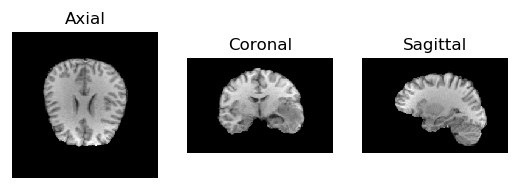
\includegraphics[scale=0.9]{brain_example}
\caption{Example cross sections of MRI flair modalities in the 2018 BraTS dataset.}
\end{figure}

\section{Methods}
\tab We created, trained and evaluated the performance of three deep-convolutional networks using a 3D U-net architecture. The models use three-dimensional convolutions with each of the four image modalities as the input image channels similar to the work of Cicek \textit{et al.} \cite{DBLP:journals/corr/CicekALBR16}. At a high level, each network has three "down" (convolution) blocks that reduce the image spatially through max-pooling, followed by three "up" (transpose convolution) blocks which combine information from the early "down" blocks to increase image dimensions to the match the ground-truth segmentation volume. The number of filters in each convolutional block increases in each successive "down" block until the model reaches its most compact representation at the lowest level with 64 filters. The number of filters then decreases with each successive "up" block until the final output has only a single channel containing the segmentation predictions.

We used skip connections to propagate relevant spatial information from early layers into the later layers. In an effort to examine trade-offs between model accuracy and efficiency, we trained three models each with different skip connections between "down" and "up" blocks. Our first model uses concatenation of "down" and "up" blocks as skip connections and does not have a dropout layer before the final output. Our second model uses element-wise summations of "down" and "up" blocks as opposed to concatenations for skip connections and includes a dropout layer, while the final model uses neither concatenations nor summations.

\begin{figure}[!ht]
\centering

\includegraphics[width=\textwidth]{model_arch}
\caption{U-net architecture of the deep convolutional network used for tumor segmentation. Each level on the three "down" blocks includes two 3D convolutional layers with "same" padding, and a max pooling layer that reduces the spatial dimensions by a factor of two. Each convolutional block uses a kernel size of $(3 \times 3 \times 3)$, and includes a batch normalization layer followed by a relu activation function (except for the final convolutional block, which uses a sigmoid activation). Each level of the "up" blocks includes a concatenation / summation layer that combines output from the respective "down" block and that of the previous "up" block. Each "up" block also includes two convolutional layers and a transpose convolutional layer with a $(3 \times 3 \times 3)$ kernel and $(2 \times 2 \times 2)$ stride which expands the spatial dimensions of the image by a factor of two. Before the final output, the summation and non-skip models were regularized via dropout on the final convolutional layers with a drop rate of $0.2$ for each node. The number of filters in the convolutional layers is $8$, $16$, $32$, and $64$ in each of the respective "down" blocks, and is mirrored in the "up" blocks. }
\end{figure}

Each model's parameters were initialized using Xavier-He initialization, optimized using Adam optimization, and use a loss function that is a derivation of the Dice coefficient. The Dice coefficient is a common metric to assess the degree of overlap between sets of pixels. For a given predicted/ground-truth segmentation $X$ and $Y$, where each tumor voxel is labeled $1$ and non-tumor voxels are labeled $0$, the dice coefficient is given by

\begin{equation}
dice(X, Y) = \frac{2 \ |X \cap Y|}{|X| \ + \ |Y|}
\end{equation}

Note that because the Dice coefficient uses the thresholded output segmentation it is non-differentiable and thus cannot be used to train the model. To solve this, we modified our loss function to create a differentiable hybrid derived from the standard dice coefficient, which is calcualted as the sum of element wise multiplications between our predicted segmentation output \textit{prior to thresholding}, $x$, and the ground-truth segmentation $Y$:

\begin{equation}
loss(x, Y) = -\frac{2 \ sum(x \times Y)}{sum(x) \ + \ |Y|}
\end{equation}

Each model was implemented in TensorFlow \cite{tensorflow2015-whitepaper} and trained for 40 epochs on a p2.xlarge EC2 instance on Amazon Web Services using a single NVIDIA K80 GPU.

\section{Experiments/Results/Discussion}

\tab In order to make valid comparisons between the three models, we ran each model with the same hyperparameters and optimizations, which were selected based on all three models' training and validation set performances. We chose Adam optimization because all three models converged to high dice scores during training much more quickly as compared to basic gradient descent. We used a batch size of one because our GPU did not have the memory capacity to store the intermediate values of more than one example during forward and backward propagation in the concatenation model.

	The U-net model requires an enormous amount of memory for training due to the huge number of intermediate values that must be stored (e.g. skip connection outputs). In particular, the original U-net architecture that we used in model 1, which uses concatenations as skip connections, requires significantly more memory than would be required otherwise. As such, in model 2 we explored the use of element-wise summations as skip connections that might preserve relevant spatial information while requiring a significantly reduced memory load, and in model 3 we forewent skip connections altogether as a basis for comparison.
    
\begin{table}[!ht]
\centering
\caption{Average dice coefficients for images from the training, test, and validation sets for each of the three models.}
\label{AvgDice}
\begin{tabular}{|l|l|l|l|}
\hline
Model         & Train ($n=205$)   & Test ($n=40$)    & Validation ($n=40$) \\ \hline
Concatenation & $0.907 \pm 0.047$ & $0.87 \pm 0.072$ & $0.89 \pm 0.07$     \\ \hline
Summation     & $0.89 \pm 0.05$   & $0.85 \pm 0.09$  & $0.87 \pm 0.08$     \\ \hline
No-skip       & $0.815 \pm 0.13$  & $0.81 \pm 0.12$  & $0.77 \pm 0.25$     \\ \hline
\end{tabular}
\label{table:AvgDice}
\end{table}

\begin{table}[!ht]
\centering
\caption{Min. and max. dice coefficients for images from the training, test, and validation sets for the three models.}
\label{MinMaxDice}
\begin{tabular}{|l|l|l|l|}
\hline
Model         & Train ($n=205$)             & Test ($n=40$)              & Validation ($n=40$)       \\ \hline
Concatenation & min $= 0.720$, max $= 0.96$ & min $= 0.67$, max $= 0.96$ & min = 0.71, max = 0.96    \\ \hline
Summation     & min $= 0.62$, max $= 0.97$  & min $= 0.48$, max $= 0.96$ & min $= 0.62$, max $=0.97$ \\ \hline
No-skip       & min $= 0.13$, max $=0.96$   & min $=0.43$, max $= 0.95$  & min $=3.7E-7$, max$=0.95$ \\ \hline
\end{tabular}
\label{table:MinMaxDice}
\end{table}
    
    Models 1 and 2 achieved stellar segmentation performance on the test set, with dice scores of $.87$ and $.85$ (Table \ref{table:AvgDice}, \ref{table:MinMaxDice}). The top performing models in recent years' BraTS Challenges have achieved whole tumor dice scores between $.85$ and $.9$, thus making our models' performances on par with the state-of-the-art. We believe that model 1's marginally superior performance is due to the enhanced access to important spatial information provided by the concatenations. However, model 2 was able to train far more quickly than model 1, and given its nearly equivalent Dice score may be a preferred implementation if storage and processing power are limited. Model 3, which contained no skip connections at all, performed significantly worse than models 1 and 2 suggesting that skip connections substantially improve performance, and furthermore that summations are an effective method of propagating skip connection information with significantly reduced computational requirements.
   We believe that our use of a hybrid dice-coefficient as a loss function also contributed subtantially to model performance. This allowed our model to optimize for a metric quite close to dice score, which is ultimately the performance metric of interest. We experimented with a cross entropy loss function and found that it yielded a far lower dice score both on training and test sets, largely due to its insensitivity towards false positives. Surprisingly, overfitting to the training data was not a substantial problem for any of our models, as indexed by average dice scores on the test and validation sets that were only slightly below that of the training set. We believe that reducing avoidable bias, as opposed to high variance, would yield far greater model improvements given the relatively small differences between training and test error and the large differences between our model's current dice score and a perfect dice score relative to the ground-truth segmentations. Due to our models' low variances, we chose not to implement regularization techniques.


\begin{figure}[!ht]
\centering

\begin{subfigure}[b]{0.5\textwidth}		
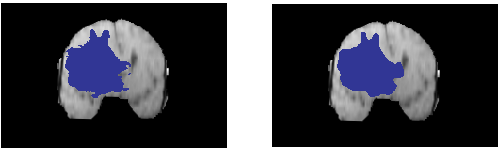
\includegraphics[width=\textwidth]{Brats18_2013_12_1_108}
\caption{Subject: "Brats18\_2013\_12\_1", Dice $= 0.93$}
\end{subfigure}

\begin{subfigure}[b]{0.5\textwidth}
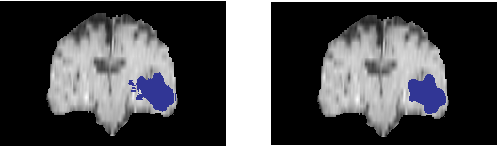
\includegraphics[width=\textwidth]{Brats18_TCIA08_406_1_127}
\caption{Subject: "Brats18\_TCIA08\_406\_1", Dice $= 0.91$}
\end{subfigure}

\begin{subfigure}[b]{0.5\textwidth}
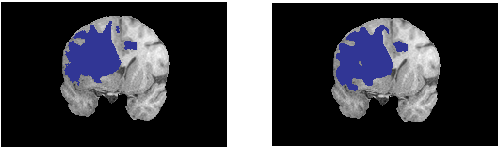
\includegraphics[width=\textwidth]{Brats18_CBICA_AUN_1_111}
\caption{Subject: "Brats18\_CBICA\_AUN\_1", Dice $= 0.93$}
\end{subfigure}

\begin{subfigure}[b]{0.5\textwidth}
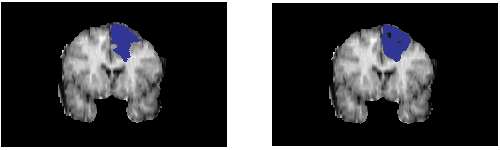
\includegraphics[width=\textwidth]{Brats18_TCIA10_420_1_97}
\caption{Subject: "Brats18\_TCIA10\_420\_1", Dice $= 0.82$}
\end{subfigure}

\caption{Axial slices of examples from the validation set showing expert-labeled (left) and predicted (right) segmentations in blue. Predicted segmentations were produced by the model with concatenated skip-connections (Model 1) Predicted segmentations tend to have smoother edges than expert-labeled tumors, but maintain the same shape and size even in tumors with many involutions. Examples where the model did not perform well, such as (d) generally do not have well-defined edges to the tumor.}
\end{figure}

\section{Conclusion/Future Work}
\tab We have shown that fully-convolutional U-net models are capable of achieving high performance on whole-tumor segmentation tasks from MR images. We found that the U-net model with concatenation skip connections yielded the highest performance but that skip-connections with summation could also be used to achieve high performance at a reduced memory footprint. We also observed that skip-connections were critical components of the U-net model because of the spatial information that they add to later layers.

To build on this work, we intend first to improve the performance of this model through a more extensive hyper-parameter search, including increasing the batch size, and tuning the learning rate, number of convolutional blocks, and max-pooling kernel size. We would also like to incorporate data from past years' BraTS challenges into the training set and apply more extensive data augmentation such as random rotations, noising, and blurring. Furthermore, we would like to incorporate a post processing step in which our model’s output parameters are passed into and tuned by a conditional random field (CRF). Finally, we are interested in applying the techniques used here to other tasks in the BraTS challenge such as tumor-core segmentation or the expected survival duration prediction task.

\section{Contributions}
Jon implemented the BraTS dataset loader and used it to perform data pre-processing, including converting the dataset to TFRecord files. Jon also created the input data pipeline which does further pre-preprocessing, augments, shuffles and batches the images in parallel at training time, using TensorFlow's Dataset API. Jon implemented the baseline UNet  model in TensorFlow and configured real-time logging to TensorBoard, and periodically saving models at the end of each epoch. Jon implemented the evaluation script which restores and evaluates saved models on the test and validation sets, producing the side-by-side images of ground-truth and model output segmentations, and average dice score calculations.


Cam acquired the BraTS dataset from University of Pennsylvania’s Center for Biomedical Imaging and Analysis, implemented the U-net model which used element wise summations as skip connections, and the model which used no skip connections. Cam implemented real time graphing of training dice scores and loss functions, as well as test dice score and loss at regular intervals throughout training via tensor board. Cam also performed hyper parameter tuning of learning rate, kernel size, filter number, dropout rate and batch norm implementation.


Both Cam and Jon contributed to the overall model design, experimentation, and analysis.

\bibliographystyle{plain}
\bibliography{references.bib}

\end{document}